% $Header$

% This file is a demonstration on how a seminar file should be
% changed to make it work with beamer.


% Copyright notice:

% Except for the changes indicated by CHANGED, this file is the original
% file texpower-0.0.9d/doc/seminardemo.tex, which is part of the
% examples of the texpower package.



% seminardemo.tex,v 1.2 2002/11/14 20:46:00 hansfn Exp
%
% TeXPower bundle - dynamic online presentations with LaTeX
% Copyright (C) 1999-2002 Stephan Lehmke
%
% This program is free software; you can redistribute it and/or
% modify it under the terms of the GNU General Public License
% as published by the Free Software Foundation; either version 2
% of the License, or (at your option) any later version.
%
% This program is distributed in the hope that it will be useful,
% but WITHOUT ANY WARRANTY; without even the implied warranty of
% MERCHANTABILITY or FITNESS FOR A PARTICULAR PURPOSE.  See the
% GNU General Public License for more details.
%
%-----------------------------------------------------------------------------------------------------------------
% File: seminardemo.tex
%
% Simple examples the for combining the seminar class with the dynamic features provided by the package texpower.sty.
%
%-----------------------------------------------------------------------------------------------------------------
% Autor: Stephan Lehmke <Stephan.Lehmke@cs.uni-dortmund.de>
%
% v0.0.1 Jun 02, 2000: First version for the pre-alpha release of TeXPower.
%


% CHANGED: commented
%\documentclass{seminar}
%
%% We need fixseminar for setting the page size correctly.
%
%\usepackage{fixseminar}
%
%
%%-----------------------------------------------------------------------------------------------------------------
%% The texpower package is loaded.
%% We give the display option so dynamic features are enabled.
%%
%\usepackage[display]{texpower}

% CHANGED: Added
\documentclass[slidestop,usepdftitle=false]{beamer}
\usepackage[accumulated]{beamerseminar}
\usepackage{beamertexpower}
\usepackage{beamerthemeshadow}
\usepackage{ragged2e}
\usepackage{graphicx} % For including images

\graphicspath{{./Images/}} % Specifies the directory where pictures are stored

% if using pdflatex:
%\setlength{\pdfpagewidth}{\paperwidth}
%\setlength{\pdfpageheight}{\paperheight}

\newenvironment{list1}{
  \begin{list}{\ding{120}}{%
      \setlength{\itemsep}{0in}
      \setlength{\parsep}{0in} \setlength{\parskip}{0in}
      \setlength{\topsep}{0in} \setlength{\partopsep}{0in}
      \setlength{\leftmargin}{0.20in}}}{\end{list}}
\newenvironment{list2}{
  \begin{list}{$\bullet$}{%
      \setlength{\itemsep}{0in}
      \setlength{\parsep}{0in} \setlength{\parskip}{0in}
      \setlength{\topsep}{0in} \setlength{\partopsep}{0in}
      \setlength{\leftmargin}{0.2in}}}{\end{list}}



% CHANGED: Moved \title and \author outside of slide
\title{{\normalfont Artificial Intelligence in Cyber Security of Cloud Based Systems: Detection, Repair and Defense}}
\author[Aytaç Özkan]{Aytaç Özkan\\\code{mailto:Aytac.Ozkan@inra.fr}}

\begin{document}
\begin{slide}

\maketitle

\newslide

\tableofcontents
\end{slide}

% CHANGED: Added \frame, moved \section out, added \frametitle
\section{About me}
\frame{
\begin{slide}
\centerslidesfalse
\frametitle{About me}

% The \pause command `splits' the current page at the place it appears, producing two pages, one with everything which
% came before the \pause command, one containing this and additionally the stuff coming after \pause. When these pages
% are presented with acrobar reader in full screen mode (or any other viewer with this capability), the presentation
% will appear to `stop' at the point the \pause command was issued and `resume' in the moment the presenter switches to
% the next page.

{\bf Universite // Paris Seine, École internationale des sciences du traitement de l'information}, Cergy, France
% {\em Faculty of Engineering}
 \vspace*{0.0in}
 \begin{list1}
 \item[] M.S., Big Data,  July, 2019
 \begin{list2}
 \item Dissertation Topic:  ``Improving data quality for big data using advanced analytics''
 \item Advisor: Prof. Rachid Chelouah
 \end{list2}
 \end{list1}

{\bf Marmara University}, Istanbul, Turquie\\
%{\em Department of Mathematics and Statistics}
\vspace*{0.0in}
\begin{list1}
\item[] M.S., Information Systems and Engineering,  May, 2017
\end{list1}
{\bf Professional Experience} \\
{\textbf{INRA}, Institut national de la recherche agronomique}, Avignon, France
{\em Research Software Engineer} \hfill {May, 2019 - present}
\end{slide}
}
\frame{
\begin{slide}
\frametitle{Ultra Marathon}
\begin{figure}
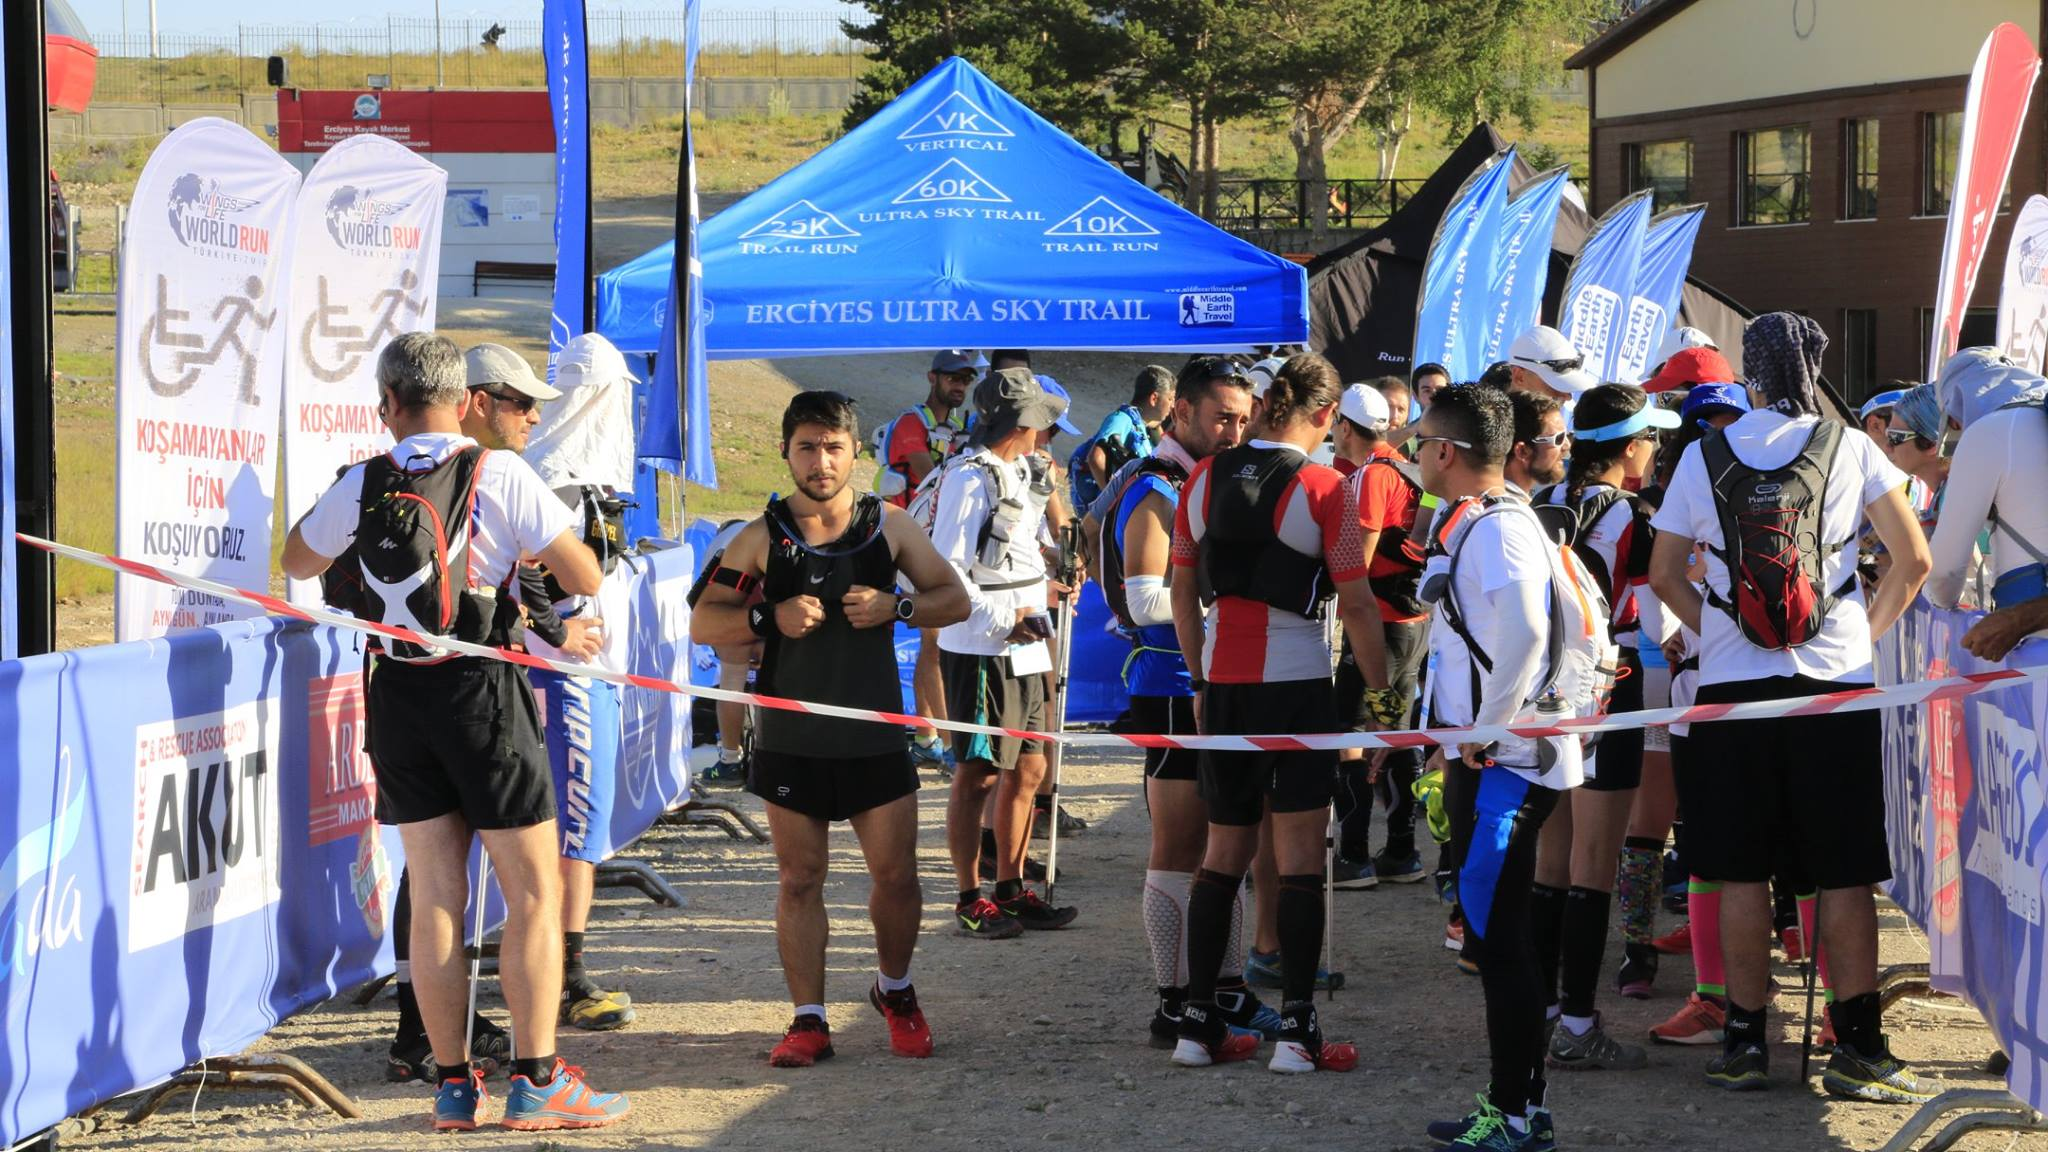
\includegraphics[width=0.9\textwidth]{erciyes_2}
\caption{Erciyes Ultra Sky Trail}
\end{figure}
\end{slide}
}

% CHANGED: Added \frame, moved \section out
\section{Motivation}
\justifying
\frame{
\begin{slide}
\centerslidestrue
\frametitle{Motivation}
The speed of process and the amount of data to be used in defending the cyber space cannot be handled by humans without considerable automation at the cloud base systems.
However, it is difficult to develop software with conventional fixed algorithms (hard-wired logic on decision making level)
for effectively defending against the dynamically evolving attacks in networks. This situation can be handled by applying methods of artificial intelligence that provide flexibility
and learning capability to software.
Computer Security system providers are unable to provide timely security update. Most security systems are not designed to be adaptive to
the increasing number of new threats. Companies lose considerable amount of time and resources when security attacks manifest themselves.
\end{slide}
}
\frame{
\begin{slide}
As a answer to these problems this research is aimed at developing security systems capable of learning and updating themselves.
The goal is to create security systems that will autonomously mature with expose to threats over time.
To achieve this goal this research is proposing artificial intelligence based security systems with learning capability
to perform intrusion, detection, repair and agnostics and defending network.
\end{slide}
}

% CHANGED: Added \frame, moved \section out
\section{AI: The next Frontier in IT Security}
\justifying
  \centerslidesfalse
\frame{
\begin{slide}
  \frametitle{AI: The next Frontier in IT Security}
  \textit{AI} in cybersecurity is a set of capabilities that allows organizations to detect, predict and respond to cyber threats in real-time
  using machine and deep learning.

  \textbf{AI-enabled cybersecurity is increasingly necessary}, organizations face an urgent need to continually ramp up and improve their cybersecurity.
    This is because the number of end user devices, networks and user interfaces continues to grow as a result of advances in cloud, the IoT,5G and conversational interfaces.
    The increases the difficulty involved with administering a computer network. Having artificially intelligent network infrastructure that can learn to detect,
    report and repair network security problems is an advantage to network administrators.
\end{slide}
}

\frame[allowframebreaks]{
\begin{slide}
Adaptability is another key reason that brought AI and computer security close to each other. The malicious entities that generate computer security attacks have gained intelligence.
The type of attacks evolved from a simple password guessing to a staged and distributed network attack that can be equipped with a stealth mode and attack that mutation.
The compute security field has to adopt to rapid change and the evolution of security attacks. AI us well situated to answer this situation. AI is concerned with creating systems that evolve
and react depending on the changes in the surrounding environment.

\textit{Fighting the Unknown}. For many years, the efforts of the IT security industry were based on the assumptions
that attacks were conducted on a large scale and major threats spread before arriving at a specific network or computer.
Solutions were created on the basis of these assumptions and addressed as fellows.
\end{slide}
}
\frame{
\begin{slide}
\textit{Internet of Things} In the past, most Internet interactions were interactions between humans that communicated via different platforms over the global network.
Communications between humans, as the primary users of online communications will change dramatically with the evolution of the IoT realm ~\cite{Ko:2016:STU:2909066.2835492}.

Most of the entities that will communicate on the Web in the future will be machines, and they will be used to initiate
reports, make contact, or respond to requests. ~\cite{Komninos:2012}
The means to facilitate this is characterized by easy access to the Web and the ability for mass distribution. For example, there is a possibility to turn households into smart homes with
intercommunicative technology instead of investing in designing a supporting infrastructure.
\end{slide}
}

\frame{
\begin{slide}
    Even scattering sensors along oil fields is the result of technological developments that led to a decrease in
the price of materials, easy logistical operation, and resistant products that meet industrial standards. ~\cite{Chen:2017:DAI:3046067.3046227}
The cyber world has barely begun to focus on new types of dangers such as the autonomous world, since this process has just started. However, the severity
level of the threat is clear. In coming years, the cyber defense community will be called upon to develop
new and effective technologies to meet the challenges posed by our changing and increasingly autonomous world.
\end{slide}
}



% CHANGED: Added \frame, moved \section out
\section{The Contribution of Intelligent Systems to Cyber Security}
\justifying
\centerslidesfalse

\frame{
\begin{slide}
\centerslidesfalse
\frametitle{The Contribution of Intelligent Systems to Cyber Security}
Artificial intelligence (AI), which was officially established in the late 1950s by scholars such as Marvin Minsky, is used as a generic name representing a wide variety of
methods, tools, and techniques that mimic “cognitive” functions or tasks that people
associate with the human mind, such as “learning,” “planning,” “reasoning,” or “problem solving” ~\cite{Russell:1995}.
The importance of AI in cyber security is twofold and related to two opposing directions. The first direction focuses on
AI-controlled systems as potential targets of cyber attacks, mainly due to their increasing role in controlling vital and complex
systems. There are numerous examples of cyber risks related to AI-controlled systems, such as smart vehicles ~\cite{Berger:2013:PLC:2489103.2514809}
, smart grids and smart cities ~\cite{ALDAIRI20171086}.
\end{slide}
}

\frame[allowframebreaks]{
\begin{slide}
\textbf{Knowledge-based systems and machine learning methods} are two well-known classes of AI methods that contain valuable tools
used in cyber security. In Knowledge-based systems, a huge amount of (experts') Knowledge is uploaded to the computer memory (thus, it is also called expert systems). ~\cite{Felgenbaum:1977:AAI:1622943.1623042}
The learning part in these systems is based on the reasoning related to this large body of knowledge, which is often obtained  by programmed rules (such as "if-then" and "inference logic rules").

Antivirus and antispam software packages ~\cite{Blanzieri:2008:SLT:1612711.1612715} represent 
straightforward implementations of expert systems in cyber security. In this case, expert knowledge (accumulated based on a large amount of transactions) regarding the procedures used
such as applied protocols, network traffic (e.g., HTTP, HTTPS, VoIP, or email), and I/O interactions with the operating system is organized systematically to protect the
users from cyber breaches. There are several papers in this issue that serve as good
examples of such expert systems ~\cite{Maltinsky:2017:NNM:3055535.3040966}.
\end{slide}
}

\section{Literature review}
\justifying
\centerslidesfalse
\frame[allowframebreaks]{
\begin{slide}
\frametitle{Literature review}
There have been several similar works done in IoT fields. Still, researchers are working in this area. Pahl et al. ~\cite{PahlA18} have
mainly developed a detector and firewall for an anomaly of IoT microservices in IoT site. 
Clustering methods like K-Means and BIRCH have been implemented ~\cite{AGGARWAL200381} for different microservices in this work. 
In clustering, different clusters were grouped in the same if the center is in the three times of standard deviation distance. 
The clustering model has been updated using an online learning technique. 
With the algorithms implemented, the overall accuracy obtained by the system is 96.3\%. 
A detailed description of a smart home system where security breaches were detected by deep learning method Dense
Random Neural Network (DRNN) ~\cite{BRUN2018458} have been introduced in ~\cite{BRUN2018458}.
\end{slide}
}

\frame{
\begin{slide}
Liu et al. \cite{LiuLLY18} proposed a detector for On and Off attack by a malicious network node in industrial IoT site. 
By On and Off attack they meant that IoT network could be attacked by a malicious node when it is in an active state or On state. 
Further- more, the IoT network behaves normal when its malicious node is in the inactive or off state. 
The system was developed using a light probe routing mechanism with the calculation of trust estimation of each neighbour node for the detection of an anomaly. 
\end{slide}
}


\frame{
\begin{slide}
Diro et al. ~\cite{DIRO2018761} discussed the detection of attack using fog-to-things architecture. 
The authors of the paper gave a comparison study of a deep and a shallow neural network using open source dataset. 
This work’s primary focus was to detect four classes of attack and anomaly. 
For four class the system got the accuracy of 98.27\% for deep neural network model and accuracy of 96.75\% for shallow neural network model. 
\end{slide}
}


\section{How organizations are benefiting from AI In cybersecurity}
\justifying
\centerslidesfalse
\frame{
\begin{slide}
\frametitle{How organizations are benefiting from AI In cybersecurity}
\textbf{AI lowers the cost to detect and respond to breaches:} Using AI for cybersecurity enables organizations to understand and reuse 
threat patterns to identify new threats. This leads to an overall reduction in time and effort to identify incidents, investigate them, and remediate threats.
Close to two-thirds of executives (64\%) say that AI lowers the cost to detect and respond to breaches. 
The reduction in cost for a majority of organizations ranges from 1\% – 15\% (with an average of 12\%).
 However, a few organizations have managed to achieve even higher cost reductions (more than 
 15\%) leading to higher benefits (see figure \ref{fig-cost-to-detect-and-respond-to-breaches}).
\end{slide}
}

\frame{
\begin{slide}
\begin{figure}
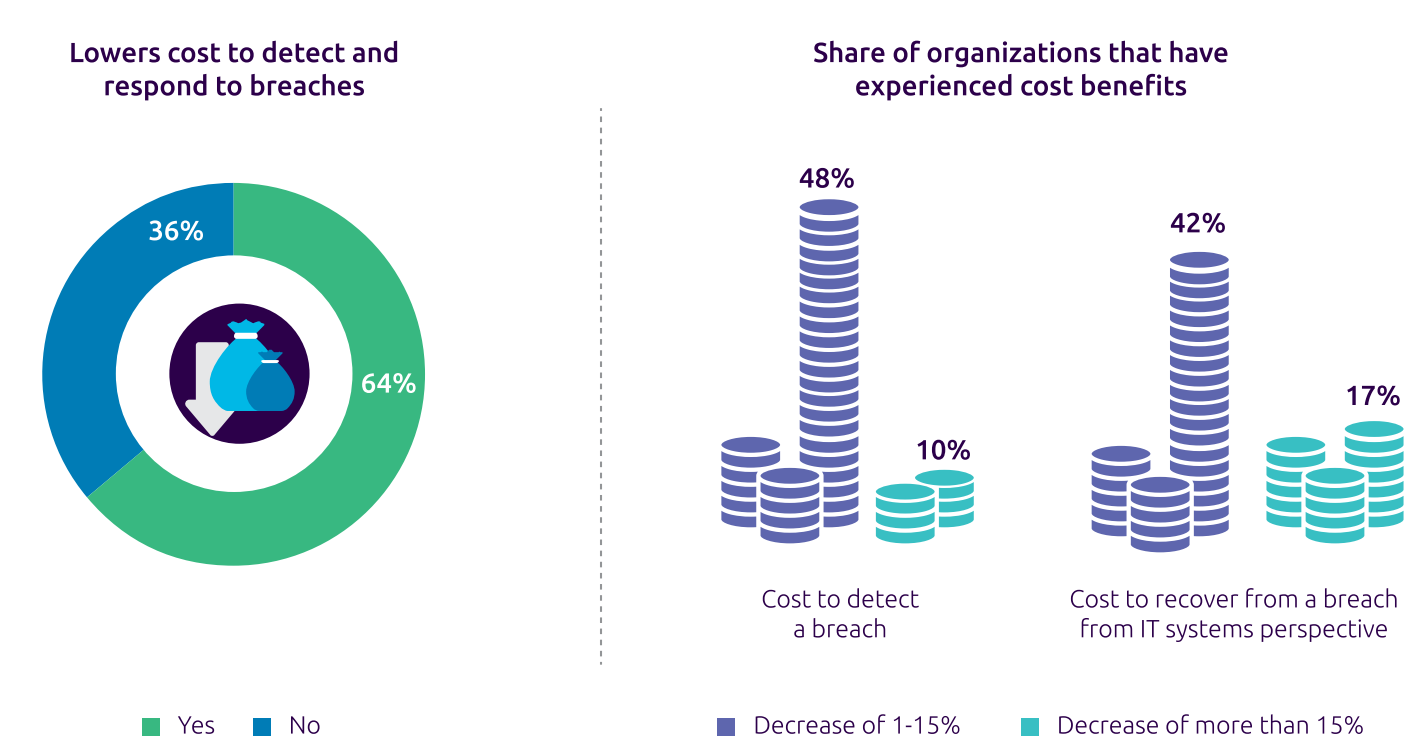
\includegraphics[width=.7\textwidth]{cost-to-detect-and-respond-to-breaches} 
\caption{AI in cybersecurity lowers the cost to detect and respond to breaches ~\cite{Capgemini2019}.}
\label{fig-cost-to-detect-and-respond-to-breaches}
\end{figure} 
\end{slide}
}

\frame[allowframebreaks]{
\begin{slide}
    \textbf{AI makes organizations faster at responding to breaches:}
    Fast response is essential to securing an organization from cyber attacks. With AI, the overall time taken to detect threats and breaches is reduced by up to 12\%. 
    AI also reduces the time taken to remediate a breach or implement patches in response to an attack by 12\%. A small subset of organizations even managed to reduce these time metrics by greater than 15\%
    zPower, a leading rechargeable battery manufacturer, partnered with a startup to use AI to detect and autonomously respond to threats as they emerge. Just weeks after the solution was deployed, 
    the security team was alerted to the fact that an employee had downloaded potentially malicious software. They were able to remove the threat and head off any attack in real time ~\cite{Darktrace2017}.
    (see figure ~\ref{fig-responding-to-breaches} \footnote{Source: Capgemini Research Institute, AI in Cybersecurity executive survey, $N$ $=$ $850$ executives})
\end{slide}
}

\frame{
\begin{slide}
\begin{figure}
    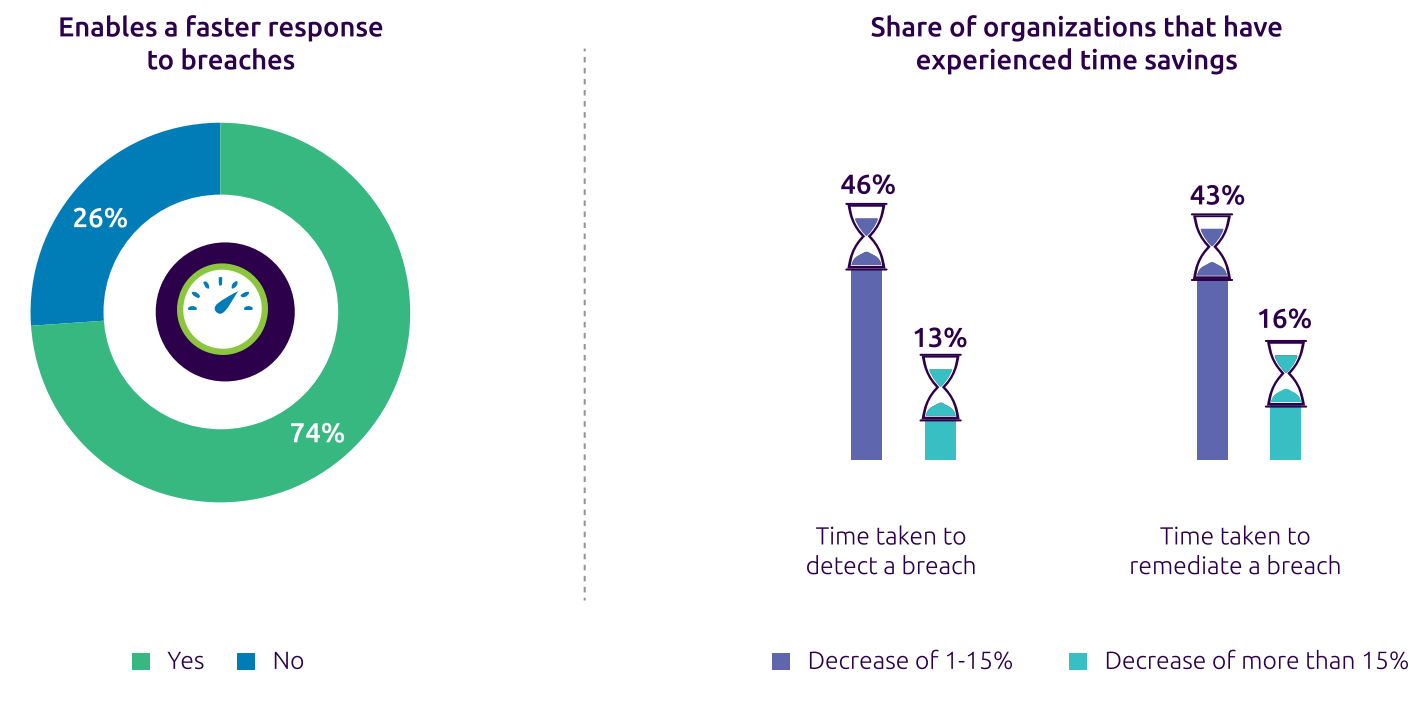
\includegraphics[width=.9\textwidth]{responding-to-breaches} 
    \caption{Nearly three in four executives say AI in cybersecurity enables a faster response to breaches
    Enables ~\cite{Capgemini2019}.}
    \label{fig-responding-to-breaches}
\end{figure} 
\end{slide}
}

\frame{
\begin{slide}
    \textbf{AI results in higher efficiency for cyber analysts:} Cyber analysts spend considerable time going through data logs and/or incident timesheets. With AI helping carry that workload, cyber analysts can spend more quality time analyzing the incidents identified by the AI cybersecurity algorithms.
\end{slide}
}

\frame{
\begin{slide}
\begin{figure}
    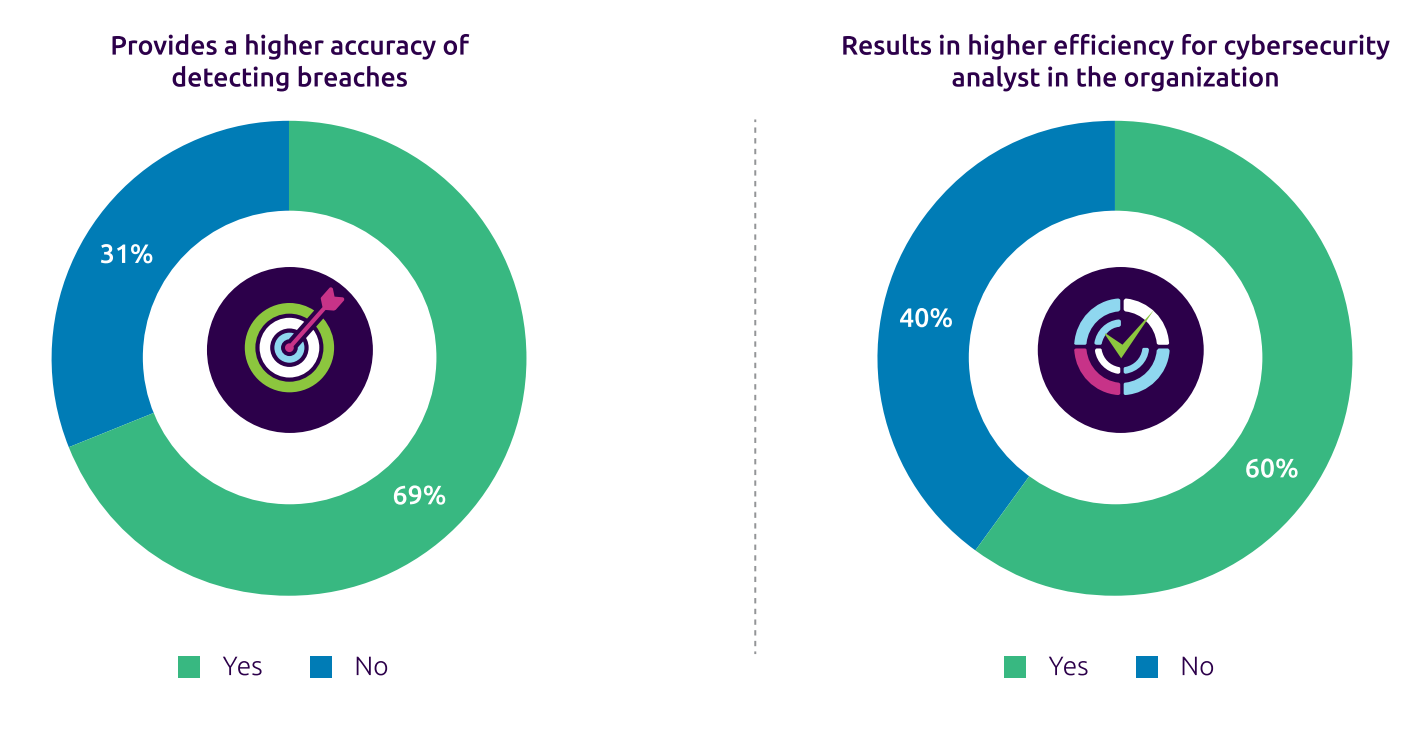
\includegraphics[width=.9\textwidth]{accuracy-of-detecting-breaches} 
    \caption{AI can help organizations provide a higher accuracy of detecting breaches
    Provides ~\cite{Capgemini2019}.}
    \label{fig-accuracy-of-detecting-breaches}
\end{figure} 
\end{slide}
}

\frame[allowframebreaks]{
\begin{slide}
    \begin{itemize}
        \item {
           \textbf{AI results in new revenue streams through cybersecurity offerings:}
           With the proliferation of smart products – electronic devices generally connected wirelessly to other devices or networks – the attack surface for hackers increases. This creates an opportunity – offering cybersecurity services to manufacturers that sell smart products. A number of organizations are already targeting this opportunity:
               \begin{itemize}
                  \item {
                    \textbf{GE’s} Digital Ghost technology offers an AI-enabled protective layer for industrial control systems. Digital Ghost leverages the digital twins (which are often referred to as the brains of the associated control systems) to gain knowledge of the machine’s working pattern. Digital Ghost detects if the machine, while appearing to operate normally, 
                    is actually being influenced by cyber attacks ~\cite{GEResearch2019}.
                  }
                  \item {
                    Similarly, \textbf{Siemens’} ‘Industry Anomaly Detection’ solution uses AI to detect anomalies, either via intrusion or data theft by hackers. The solution analyzes data traffic in the network in a learning phase to establish transparency 
                    of every device connected to the network. It can then identify any vulnerabilities while providing continuous monitoring to detect anomalies. ~\cite{Siemens20118}
                  }
               \end{itemize}  
           }
     \end{itemize}
\end{slide}
}

\section{Research Plan}
\justifying
\centerslidesfalse
\frame{
\begin{slide}
\frametitle{Research Plan} 
\vspace*{-0.2in}
\begin{figure}[h]
   \center
   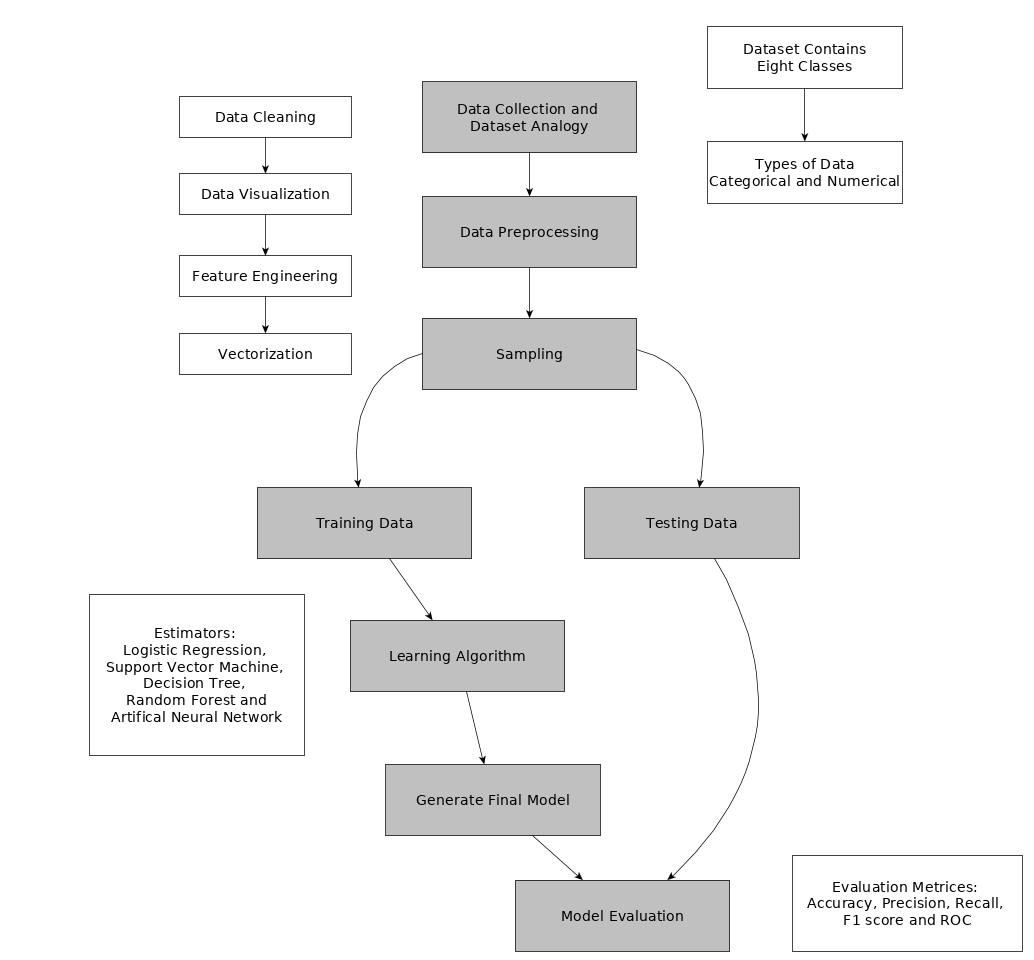
\includegraphics[width=.5\textwidth]{sec-framework-fig.png} 
   \caption{Overall framework for attack and anomaly detection in IoT and Cloud Base Services.}
   \label{fig-example}
\end{figure}
\end{slide}
}

\begin{frame}
  \frametitle{Research Plan} 
   \begin{slide}
    \begin{itemize}
        \item {
            Analyzing previous AI solutions which is developed for cybersecurity and figure out the deficiencies of the application. 
         }
        
         \item{
            Investigating "exploit databases" and collecting data related the kind of the threats.  
         }
         \item {
            Analyzing Cloud Based Systems' network infrastructures for collecting data. 
         }
        
         \item {
            Researching common and recent threats for the computer networks.
         }
     
         \item {
            Investigating the literature of the machine learning algorithms. 
        }
     \end{itemize}
   \end{slide}
\end{frame}

\begin{frame}
  \frametitle{Research Plan} 
   \begin{slide}
    \begin{itemize}
      \item {
        Investigating the literature of the machine learning algorithms. 
    }
    \item {
        Analyzing the vulnerabilities of the cloud systems.   
    }
 
     \item {
        Defining the constraints of the problem.
     }
 
     \item {
        Modeling the problem. 
     }
     \item {
        Creating the fittest machine learning models for AI application 
     }
     \item {
        Developing the AI application that can detect, repair and defense the cloud based systems to against the cyber threats and attacks.
     }
     \end{itemize}
   \end{slide}
\end{frame}

\begin{frame}
  \frametitle{Research Plan} 
   \begin{slide}
    \begin{itemize}
      \item {
        Creating real-world test environment and creating real-time cyber-attacks scenarios for test the developed AI supported security applications.
    }
 
    \item {
        Regarding the test results of the application, optimize the AI algorithms with heuristic and metaheuristic approaches.  
    }
     \end{itemize}
   \end{slide}
\end{frame}

\section{Conclusions}  
  \begin{frame}%%   
  \frametitle{Conclusions}  
  \begin{center}
  {\fontsize{42.99}{50}\selectfont Thank You!}
  \end{center}
  \end{frame}

\begin{frame}[allowframebreaks]
    \frametitle{References}
    \addtocontents{toc}{\vspace{2em}} % Add a gap in the Contents, for aesthetics
    \bibliographystyle{amsalpha}
    \bibliography{Preamble/Thesis_bibliography} % The references information are stored in the file named "Thesis_bibliography.bib"
\end{frame}
\end{document}
